94. Единственное решение имеет уравнение $x^2+p=-4x-5,\ x^2+4x+(p+5),$ значит $D=16-4(p+5)=0,\ p+5=4, p=-1.$ Тогда $x^2+4x+4=0,\ (x+2)^2=0,\ x=-2,\ y=4-1=3,$ то есть точка их пересечния имеет координаты $(-2;3).$
$$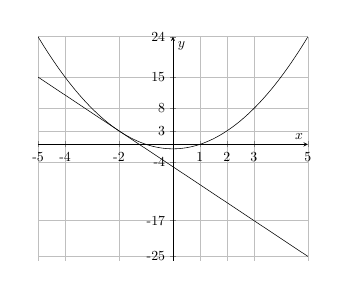
\begin{tikzpicture}[scale=0.5]
\begin{axis}[
    axis lines = middle,
    grid=major,
    legend pos={south west},
    xlabel = {$x$},
    %xlabel style={below right},
    ylabel = {$y$},
    ymin=-26,
    ymax=24,
    xmin=-5,
    xmax=5,
    xtick={-5,-4,-2, 1,2, 3, 5},
    xticklabels={-5,-4,-2, 1,2, 3, 5},
    ytick={-25,-17,-4, 3, 8, 15, 24},
    yticklabels={-25,-17,-4, 3, 8, 15, 24},
                  ]
\addplot[domain=-5:5, samples=100, color=black] {(x*x-1)};
\addplot[domain=-5:5, samples=100, color=black] {(-4*x-5)};
        %\addplot[domain=2.01:6, samples=100, color=black] {2/(2-x)};
   % \addplot[domain=-3:3, samples=100, color=black] {-x};
     %\addlegendentry{$\text{Рис. 1}$};
\end{axis}

\end{tikzpicture}$$
